% B / onlysonder：#9；本轮不修改 #4 或 #12。
\section{候选跨重复验证与复现边界}
\subsection{固定候选与比较口径}
沿用 WT rep1 的 1 kb 扫描 top 1\% 规则，阈值 0.04633597284555435，
47 个窗口按已有重叠连通分量合为 10 个独立位置。
每个位置在查看 rep2 前固定以 rep1 重建误差最高的原 24 kb 窗口作代表，并列按候选 ID。
共享 \path{src/preprocessing.py} 读取同坐标 100 bp O/E；
O/E 为 counts 除以环状距离背景，背景包含零接触对，无伪计数或逐窗口缩放。

仓库未指定相关类型，故预先选择 Pearson。
只统计两重复共同有效且有限的严格上三角像素，排除主对角线；有效零值保留。
不用模型缩放图或显示截断值计算相关。像素不足或常量数据标为无法判定；本次均未触发。
配对图共享 mask、坐标和固定 O/E 0--10 色标；灰色区域不参与统计。
对照固定为各类首条注释与 seed=20261002 的三个不与已知注释、候选及其他背景相交的窗口。
已知对照可相互重叠，只作图形参照，不视为独立统计样本。

\subsection{真实双重复统计与审阅}
10 个位置均取得相关结果，Pearson $r=0.6638$--$0.9158$，中位数 0.8572，
每个位置共同有效上三角像素为 17,578--28,680 个。
预选已知对照 $r=0.3453$--$0.3601$；背景 $r=0.1953$--$0.3489$。
这些是少量对照的描述性比较，不是显著性检验；接触像素相关，也不能作独立位置数。

\begin{table}[htbp]
\centering\small
\caption{10 个独立位置的固定代表窗口。ID 前缀均为 \texttt{candidate\_}；区间为 0-based 左闭右开。}
\begin{tabular}{lrrrr}
\toprule
ID & 比较区间（bp） & Pearson $r$ & 有效像素 & 排除像素 \\
\midrule
001 & 105000--129000 & 0.6638 & 28680 & 0 \\
006 & 1287000--1311000 & 0.8732 & 26335 & 2345 \\
011 & 2385000--2409000 & 0.8413 & 28680 & 0 \\
015 & 2720000--2744000 & 0.7385 & 19900 & 8780 \\
018 & 3256000--3280000 & 0.8771 & 28680 & 0 \\
021 & 3307000--3331000 & 0.7269 & 28680 & 0 \\
024 & 3423000--3447000 & 0.9051 & 19110 & 9570 \\
028 & 3533000--3557000 & 0.8967 & 28680 & 0 \\
035 & 4161000--4185000 & 0.7402 & 17578 & 11102 \\
046 & 4237000--4261000 & 0.9158 & 28680 & 0 \\
\bottomrule
\end{tabular}
\end{table}

逐图审阅后，10 个位置保留为可重复接触图形证据；本次未见明显整体现象不一致的代表窗口。
其中 006、015、024、035 有无效区域，只保留共同有效部分，不能判定完整窗口或全部合并区域。
035 的有效比例仅 61.29\%，其灰色缺口不能解释为接触降低。
全部成员、代表坐标、像素数及逐位置理由保存在最终审阅表；47 行衔接表的相关明确指向位置代表，
不表示 47 次独立复现。

图中示例按最高 rep1 得分候选、首个预选已知与首个背景选择，不依据 rep2 的相关排名。
候选得分此前与强度明显相关；较高相关可能包含接触密度和条带贡献，不能据此证明结构类别或生物学功能。

\begin{figure}[p]
\centering
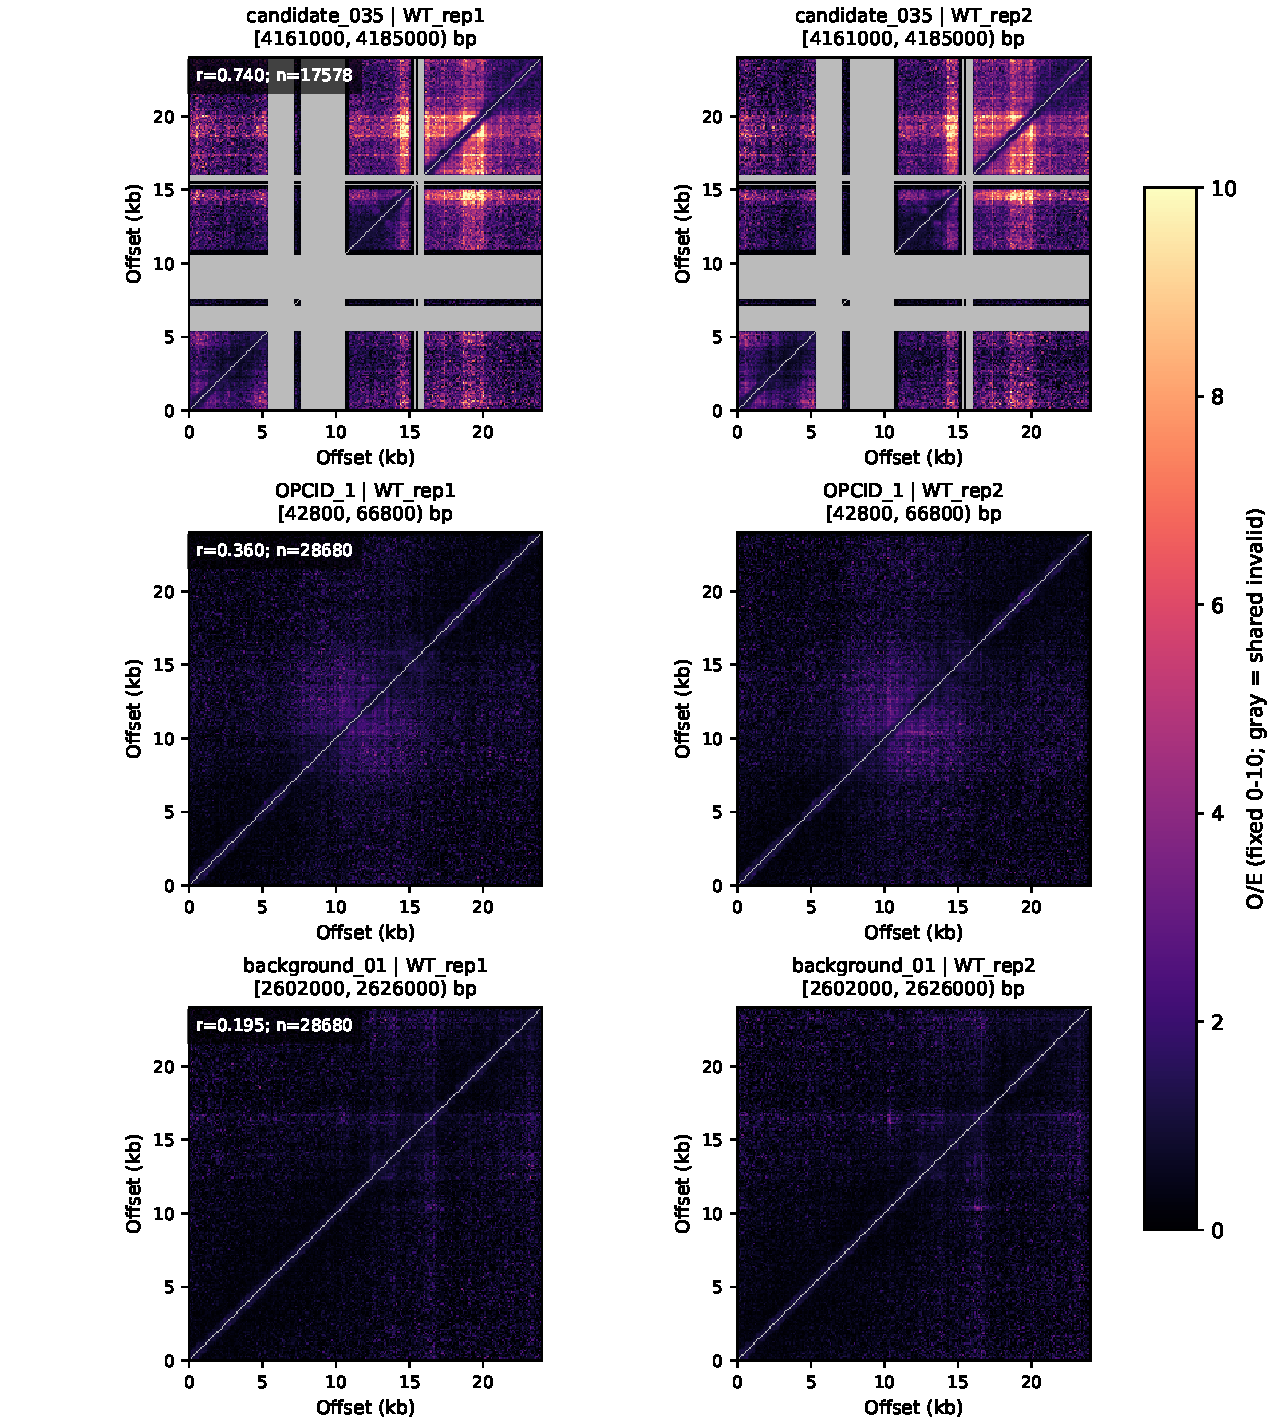
\includegraphics[height=0.76\textheight,width=0.98\textwidth,keepaspectratio]{../results/validation/paired_examples.pdf}
\caption{WT rep1/rep2 的同坐标 O/E 配对图。上：候选 035，$r=0.7402$，有效像素 17,578；
中：OPCID\_1，$r=0.3601$；下：固定背景 01，$r=0.1953$。
统一色标与共同 mask；灰色含主对角线和无效区域，不计入相关。显示截断不影响数值分析。}
\label{fig:wt-replicate-pairs}
\end{figure}

\subsection{召回与保留／排除结论}
同染色体的注释和候选半开区间有正长度交集即记为命中，跨原点按分段区间处理，
最后按结构 ID 去重。固定候选与本次保留的 10 个图形位置的注释召回均如下：
\begin{center}
\begin{tabular}{lrrr}
\toprule
类别 & 去重命中 & 已知总数 & 召回 \\
\midrule
OPCID & 10 & 68 & 14.71\% \\
CHIN & 10 & 250 & 4.00\% \\
CHID & 1 & 26 & 3.85\% \\
\bottomrule
\end{tabular}
\end{center}
合计 21/344（6.10\%）。这是保留位置的注释命中，不是对 21 条结构逐条完成复现检验。
8 个位置与已知注释重叠；015 和 035 未重叠，但仍不满足原新簇规则。
该规则要求非噪声簇至少 5 个独立候选位置、无已知参考且候选不与注释相交。
本次没有可信新结构；所有位置均排除作为“新结构发现”的依据。
没有根据 rep2 结果补选通过阈值、改候选规则或重新训练发现模型。

\subsection{输入校验与运行记录}
2026 年 10 月 2 日收到 WT 原始交接 ZIP，两个文件的名称、字节数和实测 SHA-256
均与要求一致；Cooler 为 10 bp、单染色体 NC\_000913.3、长度 4,641,652 bp、
整数 counts、无 weight。两个重复总 counts 分别为 368,695,972 与 358,452,621。
仅用包内 WT-only 清单生成 100 bp 缓存，约 124 秒；真实候选和已知结构的小样本入口先通过，再分析全部位置。
实际环境 Python 3.14.6、CPU；HEAD、代码／输入哈希、缓存命令与参数记录在
\path{docs/results/validation/}。
原始矩阵和缓存被 Git 忽略；未修改 A/C 文件，未暂存或提交。
本节只验证预选代表窗口，未穷尽 47 个成员或位置并集；三组已知／背景对照规模有限。
\#12 的独立复跑、打包与视频不在本次范围内。
